\documentclass[../main.tex]{subfiles}

\begin{document}
%%%%%%%%%%%%%%%%%%%%%%%%%%%%%%%%%%%%%%%%%%%%%%%%%%%%%%%
%   New Chapter                                       %
%%%%%%%%%%%%%%%%%%%%%%%%%%%%%%%%%%%%%%%%%%%%%%%%%%%%%%%

\chapter{Neural Networks}
In the previous chapters we met neural networks several times. We now formally introduce the basic ingredients of them and the most well-known algorithm for parameter learning, backpropagation. From several ``modern'' extensions of neural networks in the end of this chapter we will get a glimpse of the modeling power of neural networks. Neural networks have been investigated very early in late 50s and 60s as a model of computation for brains and computers. In the 80s with backpropagation and so on and so forth, neural networks succeeded in few things, and were forgot by the research community until their reemergence in around 2010 when deep learning came into play. We start with a standard model.

\section{Multilayer Perceptrons}
\subsection{An overview}
A neural network can be regard as a function that computes outputs given inputs by connected computational units. These units, also refer to neurons, are parametrized by some adaptable weights that can be learned. Each unit implements only a basic operation: a generalized linear function combined with a non-linear activation function. So to speak, each unit computes a non-linear function consisting of
\begin{equation*}
{\rm linear\ function}:\ \mathbb{R}^n\rightarrow \mathbb{R}\ +\ \text{non-linear activation function}\ \sigma:\mathbb{R}\rightarrow \mathbb{R},
\end{equation*}
where we use linear functions for their simplicity. The non-linear activation function $\sigma$ is usually fixed and not adaptable. There are several popular choices of $\sigma$, but in a particular neural network people usually only use one type of $\sigma$. The reason to use this kind of combination to encode non-linearity rather than allow any non-linear function is because we want to keep things as simple as possible in terms of each computational unit (recall that we have the flexibility in connecting them). It is also proved that neural nets with fixed simple activation functions can approximate any non-linear function arbitrarily well. Mathematically, each unit is parametrized with weight ${\bf w}\in \mathbb{R}^{n+1}$, and computes
\begin{equation*}
f^{\sigma}({\bf x},{\bf w}):=\sigma\left(w_0+\sum_{i=1}^{n}w_ix_i\right)=\sigma({\bf w}^T{\bf x})
\end{equation*}
as shown in Figure \ref{fig_7_1}, where in the last equality we ignore or absorb (rewrite ${\bf x}\rightarrow (1,{\bf x})$) bias parameter $w_0$ for clarity.
\begin{figure}[h] 
	\centering 
	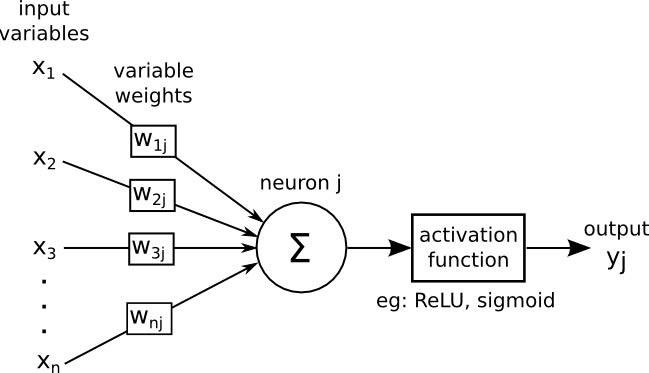
\includegraphics[width=8cm]{fig_7_1.jpg} 
	\caption{A schematic view for a unit in neural networks}\label{fig_7_1}
\end{figure}
\subsection{Activation function}
Despite the arbitrariness of choosing activation functions, there are two types of functions that are mostly used: the old school choice, logistic function (left of Figure \ref{fig_7_2}), and the new school choice, ReLU (rectified linear unit) (right of Figure \ref{fig_7_2}).
\begin{figure}[h] 
	\centering 
	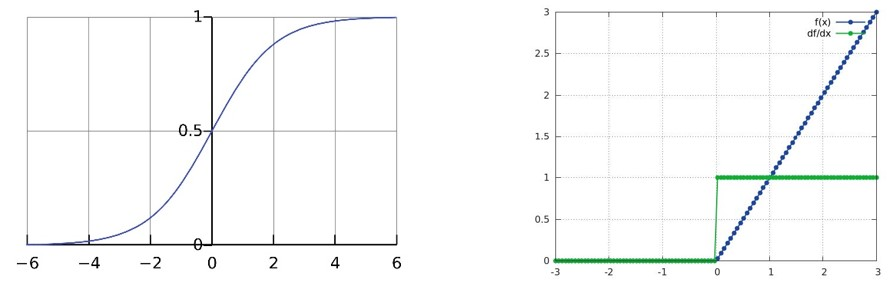
\includegraphics[width=12cm]{fig_7_2.jpg} 
	\caption{Left: logistic function. Right: ReLU.}\label{fig_7_2}
\end{figure}
\par The logistic function (left of Figure \ref{fig_7_2}), also called sigmoid function because of its shape, is given by
\begin{equation*}
{\rm sigmoid}(x) = \frac{1}{1+\exp(-x)}.
\end{equation*}
Note that it can be regard as the same function as $\tanh$ up to a rescaling and shifting since
\begin{equation*}
\tanh(x)=\frac{e^{x}-e^{ -x}}{e^{ x}+e^{ -x}} = 2\frac{e^{ x}}{e^{ x}+e^{ -x}} -1=2\frac{1}{1+e^{-2{ x}}} - 1= 2 {\rm sigmoid}(2{ x})-1.
\end{equation*}
\par The logistic function has the property that $x\rightarrow \infty,\sigma(x)\rightarrow 1$ and $x\rightarrow -\infty,\sigma(x)\rightarrow0$. This has a motivation from biology side where this type of saturate effect (maximal level of activity and inactivity) is quite common. Also mathematically speaking, the logistic function is a smooth version of the ``switch'' function, where by smooth it means differentiable up to any order, and thus has many nice mathematical properties.
\par On the other hand, ReLU (right of Figure \ref{fig_7_2}) appears to be a simpler and more straightforward function defined by
\begin{equation*}
{\rm ReLU}_{\bf w}({\bf x})=\max(0,{\bf w}^T{\bf x}),
\end{equation*}
where as its name rectified linear unit suggests it is a unit parametrized by weight ${\bf w}$. The non-linear activation function of ReLU is just given by $\max(0, x)$. ReLU is a linear function over half-space $\mathcal{H}=\{{\bf x}:{\bf w}^T{\bf x}>0\}$ and zero on its complement $\mathcal{H}^c=\mathbb{R}-\mathcal{H}$. Different from the logistic function, it's non-smooth, but simple derivatives over $\mathbb{R}-\{0\}$. Therefore, to some degree, we can say that the ReLU function has minimal non-linearity.
\subsection{Multilayer Perceptron}
With a model for each unit, we can put these neurons together to form a computational graph where we do this in terms of layers (Figure \ref{fig_7_3}). Although we have the freedom to make (directed) connections quite arbitrarily as long as there's no loop, which is essential for these graphs to be computable, this layer architecture gives a rather simple but still adaptable model enough for exploring. 
\begin{figure}[h] 
	\centering 
	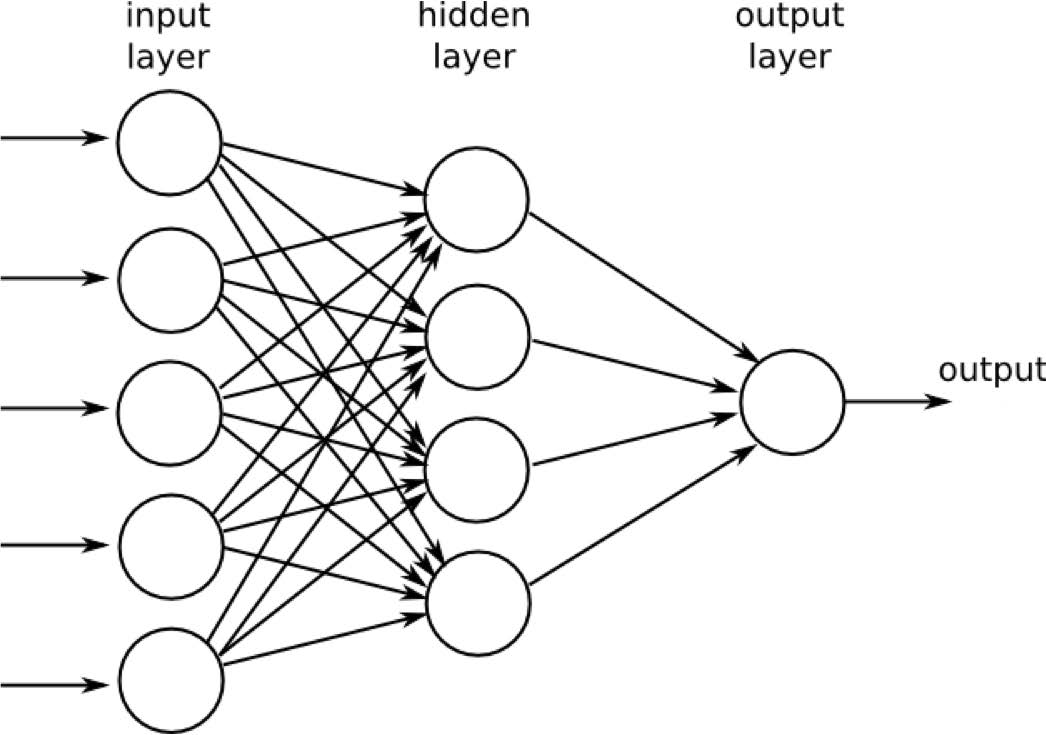
\includegraphics[width=6cm]{fig_7_3.jpg} 
	\caption{A typical structure for neural networks.}\label{fig_7_3}
\end{figure}
\par Typically, the first layer is the raw input ${\bf x}$, where no computation is involved; the last layer serves as the final output whose form depends on specific task (class label for image classification). Although what the input and the output should be is clear in this case, we have no idea about what the intermediate layers represent, and how to learn the weights becomes a big question. To start our discussion, we first build up some useful notations.
\par As mentioned above, we arrange units in layers. With units indexed by $j$ and a shared choice of $\sigma$, we can write the (fully connected) mapping between two layers in a vector form
\begin{equation*}
F^{\sigma}:\ \mathbb{R}^n\rightarrow \mathbb{R}^m,\ F^{\sigma}_{j}({\bf x})=\sigma({\bf w}_j^T{\bf x}),\ j=1,\dots,m,
\end{equation*}
where $n$ and $m$ represent the number of units of the previous/old and the current/new layer respectively; ${\bf x}$ can be the input or activation of the previous layer, and $ F^{\sigma}_{j}$ denotes a unit in the current layer. We can also take one step further to make everything in a matrix-vector notation ($\sigma$ is applied elementwise):
\begin{equation*}
F^{\sigma}({\bf x};{\bf W})=\sigma({\bf Wx}),\ {\bf W}=({\bf w}_1,\dots, {\bf w}_m)^T.
\end{equation*}
If we index layers by $l$, the activation vector of $l$-th layer by ${\bf x}^{(l)}$, we get a indexed notation for layer-to-layer forward propagation in the form of
\begin{equation*}
{\bf x}^{(l)}=\sigma^{(l)}({\bf W}^{(l)}{\bf x}^{(l-1)}),\ {\bf W}^{(l)}\in \mathbb{R}^{n_l\times n_{l-1}},
\end{equation*}
where ${\bf W}^{(l)}$ is the weight matrix between layer $l-1$ and layer $l$; ${\bf x}^{(1)}$ is the input; ${\bf x}^{(L)}$ is the output, and ${\bf x}^{(l)}$ $(1<l<L)$ are the hidden layers. \par With these notations, we can represent a $L$-layer network with a nested function given by
\begin{equation*}
{\bf y} = \sigma^{(L)}\left({\bf W}^{(L)}\sigma^{(L-1)}\left(\cdots\left({\bf W}^{(2)}\sigma^{(1)}\left({\bf W}^{(1)}{\bf x}^{(1)}\right)\right)\cdots\right)\right).
\end{equation*}
There 2 important degrees of freedom for our layer architecture:
\begin{itemize}
	\item Layer width: a wider layer means ``more of the same'' feature since the units in the same layer have the same input, the activation from the previous layer or the input.
	\item Network depth: different from the layer width, a deeper network allows ``more compositionality'' meaning that the network can have more ability to combine things and thus capture complex things. By using a deep network, we form a feature hierarchy.
\end{itemize}
\par The output layer, as mention before, depends on that type of problem we want to solve, where we may not want to naively apply the same activation function as previous layers. To simplify the notation, we have ${\bf W} = {\bf W}^{(L)},\ {\bf x}={\bf x}^{(L-1)}$. For a linear regression task, it's convenient to simply have a linear activation:
\begin{equation*}
{\bf y}={\bf Wx}.
\end{equation*}
While for a binary classification task, we want only one output ranging from 0 to 1 to form a valid conditional probability distribution. Then the logistic function can be a reasonable choice:
\begin{equation*}
y_1 = P(Y=1|{\bf x})=\frac{1}{1+\exp[-{\bf w}^T {\bf x}]}.
\end{equation*}
For the multiclass case with $K$ classes, soft-max function is usually the top choice:
\begin{equation*}
y_k = P(Y=k|{\bf x})=\frac{\exp[{\bf w}_k^T {\bf x}]}{\sum_{j=1}^{K}\exp[{\bf w}_j^T {\bf x}]}.
\end{equation*}
\par At this point, it is worth spending some time take a look at the multilayer perceptron and logistic regression in terms of classification methods. In logistic regression, we compute a linear function of inputs and map it to $(0,1)$:
\begin{equation*}
P(Y=1|{\bf x})=\frac{1}{1+\exp[-\langle{\bf w,x}\rangle]},
\end{equation*}
where ${\bf x}$ can be the original input or some learned better representations. While a multilayer perceptron first tries to learn intermediate feature representation and then perform logistic regression on learned representation ${\bf x}^{(L-1)}$. In a word, logistic regression is about: give me good representations I tell you how to linearly separate things, where logistic regression do nothing about the representations. Multilayer perceptron can learn different representations and applies logistic regression to give outputs.
\subsection{Loss Function}
Before we move forward to the learning algorithm, let us first think about what in the model needs to be learned. Things like model architecture (including the number of layers, the number of units in each layer, etc.) and the activation function $\sigma$ are our choices. We desire algorithms to learn the weights, i.e. algorithms that can automatically fiddling with network weights. 
\par The idea is to make the learning problem an optimization problem. To do so, we first need to define a \textbf{loss} function $l(y^*;y)$, where $y^*$ and $y$ are the target output and prediction respectively. Again, the form of loss function depends on the nature of the task. For a regression problem, where $y^*,y\in \mathbb{R}$, we might want to use a squared loss
\begin{equation*}
l(y^*;y)=\frac{1}{2}(y^*-y)^2.
\end{equation*}
For a binary classification task, we might desire the cross-entropy loss
\begin{equation*}
l(y^*;y)=-y^*\log y-(1-y^*)\log(1-y),
\end{equation*}
where $0\leq y\leq 1$ is used to model a Bernoulli distribution; $y^*\in \{0,1\}$ or $\in [0,1]$ (when $y^*\in [0,1]$ is a real number, this has the interpretation as a soft target encoding the uncertainty about the labeling). There is a close relationship between the cross-entropy loss and the log-likelihood. In general, the cross-entropy $H(p,q)$ measures the difference between distributions $q$ and $p$:
\begin{equation*}
H(p,q)=-\mathbb{E}_p[\log q]=-\sum_{x\in\mathcal{X}}p(x)\log q(x)\ (\text{discrete case}).
\end{equation*}
For a classification problem, if the predicted probabilities are $q_i$, while the frequency (empirical probability) of $i$ in the training set is $p_i$, and there are $N$ independent samples in the training set, then the likelihood of the training set is
\begin{equation*}
\prod_{i}(\text{probability of }i)^{\text{number of occurences of }i}=\prod_{i}q_i^{Np_i}.
\end{equation*}
So the log-likelihood, divided by $N$ is
\begin{equation*}
\frac{1}{N}\log \prod_{i}q_i^{Np_i}=\sum_i p_i\log q_i=-H(p,q).
\end{equation*}
For a single point in a binary classification problem, $p\in \{y^*,1-y^*\}$ and $q\in \{y,1-y\}$, then we have
\begin{equation*}
H(p,q) = -\sum_i p_i\log q_i=-y^*\log y-(1-y^*)\log(1-y).
\end{equation*}
When we generate $y$ with logistic function, the cross-entropy loss sometimes also refers to negative logistic log-likelihood. 
\begin{figure}[h] 
	\centering 
	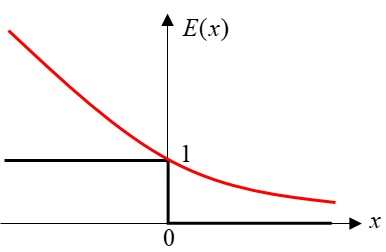
\includegraphics[width=6cm]{fig_7_4.jpg} 
	\caption{The plot of misclassification error (black) and cross-entropy loss (red) for $y^*=1$. The cross-entropy is rescaled by a factor of $1/\ln 2$, so that it pases trough the point $(0,1)$, and $x$ is the input for logistic function, i.e. $y=1/(1+\exp[-x])$.}\label{fig_7_4}
\end{figure}
\par The cross-entropy loss can be regarded as a differentiable approximation or surrogate to the misclassification error as illustrated in Figure \ref{fig_7_4}, and can never reach 0 when logistic function is applied.
\par With a loss function, we can define the objective of the optimization task for parameter learning. Specifically, given a training set of examples $\mathcal{X}-\{({\bf x}_t,y):t=1,\dots,T\}$, we'd like to minimize the empirical risk (average loss on the training data) given by
\begin{equation*}
\mathcal{L}(\theta;\mathcal{X})=\frac{1}{T}\sum_{t=1}^{T}l(y_t;\underbrace{y({\bf x}_t;\theta)}_{\text{NN output}}),\ \theta=\left({\bf W}^{(1)},\dots,{\bf W}^{(L)}\right).
\end{equation*}
Sometimes people apply regularization to make networks generalize better. Briefly speaking, by adding regularization we add prior knowledge (not depends on data) like we favor models with small weights, which is believed to be able to relieve overfitting. As an example, we can add $L_2$ regularization or ``weight decay'', which favors smaller weights, and get a regularized risk minimization objective:
\begin{equation*}
\mathcal{L}_{\lambda}(\theta;\mathcal{X}) = \mathcal{L}(\theta;\mathcal{X}) + \frac{\lambda}{2}\|\theta\|^2.
\end{equation*} 
The name ``weight decay'' comes from the fact that with $L_2$ regularization, the weights get shrunk by a factor in each gradient descent update as we will see in the following sections. Besides $L_2$ regularization, we also use many modern variant, such as drop out (training with noise), where we remove units at random during the training phase. Drop out prevents model from specialize too much.
\section{Backpropagation}
Typically the loss function is non-convex and has no closed-form optimal solutions. Gradient descent method then becomes the workhorse for most of neural network training tasks. However, because of the non-convexity of loss functions, gradient descent methods in this case have no or little theoretical guarantees. Nevertheless, in practice we ``just do it'', and it works out fine in most cases, while we might suffer from problems caused by poor local minima and saddle points, where the latter one can be more of an issue.
\par Since for large data set simply applying the steepest descent is too expensive, stochastic gradient descent (SGD) is a more popular choice. SGD with step size $\eta$ and $L_2$ regularization with $\lambda$ picks one data point $t$ at one time (it can also be multiple points, i.e. minibatch):
\begin{equation*}
\theta\leftarrow \underbrace{(1-\eta\lambda)}_{\text{weight decay}}\theta - \eta\nabla_{\theta}l(y_t^*;y({\bf x}_t;\theta)).
\end{equation*}
The problem we are left with is how to compute the gradients with respect to the weights for a large (many units) and deep (many layers) networks efficiently. This means we have to compute the partial derivative (sensitivity of outputs/loss with regard to each weight) for each weight. Thanks to the layer architecture, we can do this simply by applying the chain rule.
\par Let us start the computation from the output layer. To compute the derivative w.r.t. the outputs, we just take gradient of the loss function:
\begin{equation*}
\nabla_{\bf y}l = \dots\ \text{(depends on loss)}.
\end{equation*}
For 1-dimension squared loss, for example, we have
\begin{equation*}
\nabla_{y}=\frac{\partial l}{\partial y}=(y-y^*).
\end{equation*}
\par To determine how weights affect the output, we look from one layer back each time and evaluate how will these weights change the outputs, and ultimately we can compute the derivative w.r.t. all weights by applying the chain rules. To make this idea concrete, we take a local view with ${\bf x}$ to be the previous layer activation and ${\bf x}^+$ to be the next layer activation. How ${\bf x}$ affect ${\bf x}^+$ can be formalized by the Jacobian matrix ${\bf J}=(J_{ij})$ of mapping ${\bf x}\rightarrow{\bf x}^+,\ {x}^+_i = \sigma({\bf w}_i^T{\bf x})$:
\begin{equation*}
{\bf J}=\frac{\partial {\bf x}^+}{\partial {\bf x}},\ J_{ij}=\frac{\partial x_i^+}{\partial x_j}=w_{ij}\cdot \sigma'({\bf w}_i^T{\bf x}),
\end{equation*}
which is essentially a modified weight matrix. We see that how the change of ${\bf x}_j$ affect ${\bf x}^+_i$ will be proportional to the original weight $w_{ij}$ linking them and the ``sensitivity'' of unit ${\bf x}^+_i$ measured by $\sigma'({\bf w}_i^T{\bf x})$. Then idea of ``sensitivity'' can be understood by looking at the example of logistic activation (Figure \ref{fig_7_2}), where if $|{\bf w}_i^T{\bf x}|$ is large, the corresponding absolute value of gradient will be small and insensitive to the change of ${\bf x}$. Note that if ${x}^+_i = {\bf w}_i^T{\bf x}$ (no activation), then the Jacobian matrix will simply be the weight matrix ${\bf W}$.
\par Since the units in layer $(l-n),\ 1\leq n<l$ can only influence layer $l$ through layer $(l-1)$ (no direct connection), we can compute derivatives across multiple layers by chain rule:
\begin{equation*}
\frac{\partial x_i^{(l)}}{\partial x_j^{(l-n)}} = \sum_{j}\frac{\partial x_i^{(l)}}{\partial x_i^{(l-1)}} \frac{\partial x_i^{(l-1)}}{\partial x_i^{(l-n)}} =  \sum_{j} J_{ij}^{(l)} \frac{\partial x_i^{(l-1)}}{\partial x_i^{(l-n)}}.
\end{equation*} 
Use the result we have derived for adjacent layers, we have
\begin{equation*}
\frac{\partial {\bf x}^{(l)}}{\partial {\bf x}^{(l-n)}} = {\bf J}^{(l)}\cdot \frac{\partial {\bf x}^{(l-1)}}{\partial {\bf x}^{(l-n)}}={\bf J}^{(l)}\cdot {\bf J}^{(l-1)}\cdots {\bf J}^{(l-n+1)},
\end{equation*}
which means we only need to multiply (layer-to-layer) Jacobians. Together with the gradient w.r.t. the output, we get
\begin{equation}\label{eq_7_bp_x}
\nabla_{{\bf x}^{(l)}}^Tl=	\underbrace{\nabla_{{\bf y}}^Tl\cdot {\bf J}^{(L)}\cdots {\bf J}^{(l+1)}}_{\longrightarrow\ \text{back propagation}}.
\end{equation}
To determine how weights affect the loss, we consider again where the weights come into play. Since $w_{ij}^{(l)}$ only change unit ${x}_i$ in layer $l$ directly, all we need is a simple local computation by chain rule
\begin{equation*}
\frac{\partial l}{\partial w_{ij}^{(l)}}=\frac{\partial l}{\partial x_i^{(l)}}\frac{\partial x_i^{(l)}}{\partial w_{ij}^{(l)}},
\end{equation*}
where the first term we have already known in (\ref{eq_7_bp_x}). The second term is
\begin{equation*}
\frac{\partial x_i^{(l)}}{\partial w_{ij}^{(l)}} = \underbrace{\sigma'\left(\left[{\bf w}_i^{(l)}\right]^T{\bf x}^{(l-1)}\right)}_{\text{sensitivity of down-stream unit}}\underbrace{x_j^{(l-1)}.}_{\text{activation of up-stream unit}}
\end{equation*}
Since we can save the Jacobians along the back propagation, the cost will be roughly the same as a forward propagation. Modern tools like Tensorflow allows to build models with differentiable units and uses the built computational graph together with the chain rule to compute the gradients automatically. We see that, compared with computing the gradients for each weight separately, the symbolic calculation like what we have done can save time and cost by avoiding redundant computation.
\section{Convolutional Neural Networks}
An important observation for model designing in machine learning is that no learning machine can do well on all problems. As a results, we need to constrain our function class appropriately according to different tasks. For vision tasks, the convolutional neural networks are among the most powerful models. The idea comes from the fact that image data is in a way that often translation invariant. For example, the same type of objects should be roughly the same no matter it is in the right or left corner of an image. Therefore, we desire a kind of models that has a topological connectivity which
\begin{itemize}
	\item encourages network to first extract localized features (ignore a little bit about the location);
	\item allows subsequent layers to extract less and less localized features.
\end{itemize}
The idea is to look at a local receptive field and shift all over the image, where we compute the same thing (use the same function) at different locations. The idea of ``the same function'' is exactly the idea of weight sharing, and can dramatically decrease the parameter-to-data ratio comparing with a fully connection. With this type of design we have shift-invariant filters allowing the model to exploit the translation invariance of images. Since the discussion of how these filters actually work is rather simple but quite tedious, we skip this part and recommend readers to refer to the slides where one can find more figure illustration.
\end{document}